\documentclass[a4paper]{article}

\usepackage{amsmath, blindtext, float, graphicx, hyperref}
\graphicspath{ {./images/} }
\title{Semi-supervised sequence tagging with bidirectional language models}
\author{Shubham Gupta}

\begin{document}
\maketitle
\section{Introduction}
\begin{itemize}
    \item This is the TagLM paper mentioned in Lecture 13 in the CS224N course.
    \item This paper demonstrates how we can use context embeddings from BiLSTM models and use it for sequence labelling tasks
\end{itemize}
\section{Paper Introduction}
\begin{itemize}
    \item Typically, RNN are used only on labelled data to learn the context embeddings of words.
    \item Semi supervised approach used in this paper.
    \begin{itemize}
        \item Train LM on large unlabelled corpus
        \item Compute embedding at each position in the sequence(LM embedding)
        \item Use embedding in supervised sequence tagging model
    \end{itemize}
    \item Using both forward and backward embeddings gives better performance than using forward only LM.
\end{itemize}
\section{TagLM}
\subsection{Overview}
\begin{itemize}
    \begin{figure}[H]
        \centering
        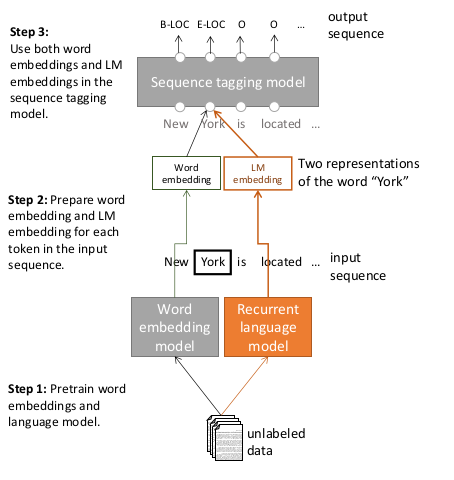
\includegraphics[width=0.8\textwidth]{main_components}
        \caption{Main componenets in the TagLM model}
        \label{fig:main_components}
    \end{figure}
    \item Extract word and LM embeddings for every token
    \item Prepare embedding by concatinating both embeddings
    \item se them in supervised sequence tagging model
\end{itemize}
\subsection{Baseline}
\begin{itemize}
    \item Baseline model is hierachical neural tagging model
    \item Obtain word and character embeddings. Concatenate them to form final embedding. $x_k = [c_k;w_k]$
    \item Char embedding: Can be obtained via CNN or RNN
    \item Word embedding: Use pretrained embeddings
    \item Use multiple bidirectional RNN to learn context embedding
    \item For every token, concatenate forward and backward hidden states at each layer
    \item 2nd layer will use the above output and predict next hidden state
    \item Use GRU or LSTM depending on task
    \item Use output of final layer to predict score for each possible tag using dense layer
    \item Better to predict tags for full sequence than for a single token
    \item THEREFORE, add another layer with params for each label bigram
    \item Compute sentence conditional random field loss(CRF) using forward-backward algorithm
    \item Use Viterbi algorithm to find most likely sequence
    \begin{figure}[H]
        \centering
        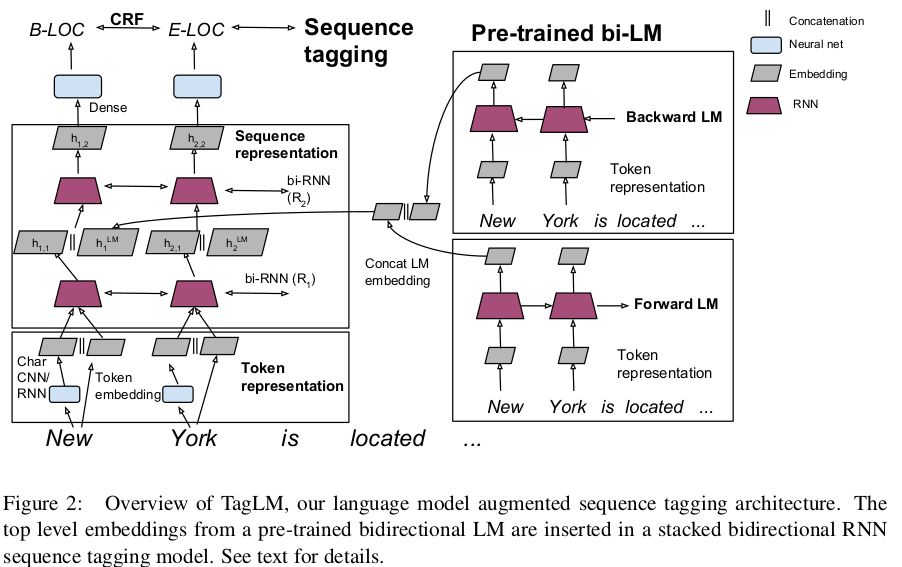
\includegraphics[width=0.8\textwidth]{overview}
        \caption{Overview of architecture}
        \label{fig:overview}
    \end{figure}
    \item LM embedding will be created by concatenating forward and backward embeddings. No param sharing between these two embeddings
\end{itemize}
\section{Experiments}
\begin{itemize}
    \item Evaulation done on CoNLL 2003 NER and CoNLL 2000 chunking
    \item Lot of detail around model architecture and training methods. Skipping this for now.
\end{itemize}
\subsection{Analysis}
\begin{itemize}
    \item Second RNN captures interactions between task specific context
    \item Backward LM addition has significant performance gains
    \item Model size makes a difference. Using bigger CNN model lead to ~0.3 percent improvement
    \item Also tried training the model JUST ON THE CoNLL data. Reduced model size
    \item Including embeddings from this model \textbf{decreased} performance compared to baseline system.  
    \item Replacing task specific RNN with using LM embeddings with a dense layer and CRF \textbf{reduced} performance 
    \item Improvement shown by transferring knowledge from other tasks \textbf{almost disappers} when the initial model is trained on a large dataset. TLDR: Moar data => Moar performance gain 
\end{itemize}
\end{document}
